\chapter{命题逻辑命题的证明}
\label{chap:sat}

\section{输入语言}
\begin{figure}[!htbp]
  \centering
  \begin{tabular}[rcl]{rcl}
    & & $Y$是原子公式 \\
    $\Pi$ & \sep{} & $Y$ \deli{} $\lnot \Pi$ \deli{} $\Pi \impl \Pi$ \deli{} $\Pi \land \Pi$ \deli{} $\Pi \lor \Pi$ \\
  \end{tabular}
  \caption{命题逻辑语言}
\end{figure}
本部分接收的语言是纯一阶逻辑命题的命题框架。命题框架是指,不理会原子公式的具体结构,只是简单地将不同的原子公式看作不同的命题变元。

\section{结构}
\begin{figure}[!htbp]
  \centering
  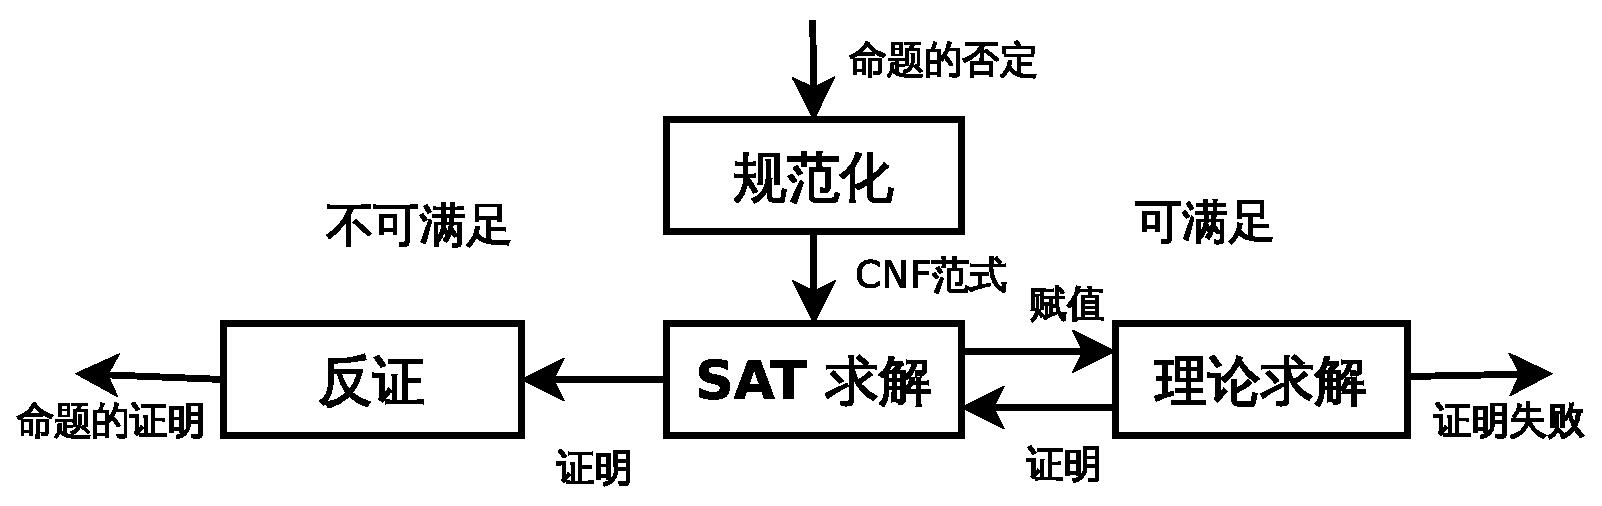
\includegraphics[width=0.8\textwidth]{sat-stru.eps}
  \caption{命题逻辑证明的结构}
  \label{sat:stru}
\end{figure}
如图\ref{sat:stru},本部分的核心是一个SAT求解器。

SAT求解器能够解决下列一类问题:

\begin{definition}[SAT问题]
设X是布尔变量集,$|X|=n$,$\alpha$是合取范式,并有$\alpha = \bigwedge_i (\bigvee_{j_1} x_{ij_1} \lor \bigvee_{j_2} \lnot x_{ij_2})$,$x_{ij} \in X$。

求一种赋值方法$(b_1, b_2, \dots, b_n)$,使得$\alpha$为真。若不存在这种赋值方法,则称$\alpha$不可满足。
\end{definition}

我们使用下面的定理来利用SAT求解器证明定理:

\begin{theorem}
  若$\lnot \alpha$不可满足,则$\vdash \lnot \lnot \alpha$。
\end{theorem}

待证的命题首先被否定并化为合取范式(CNF)$\alpha'$,然后送往SAT求解器求解。SAT求解器有可能返回两种结果:可满足和不可满足。

若结果为不可满足,如图\ref{sat:stru}左半部分,则说明$\vdash \lnot \lnot \alpha$,直接将SAT求解过程的证明证明项取出,并应用在Coq定义的双重否定引理:
\begin{verbatim}
  Lemma NNPP : forall p:Prop, ~ ~ p -> p.
\end{verbatim}
即可得证。

若结果为可满足,如图\ref{sat:stru}右半部分,将得到一个原子命题的赋值向量$\vec{v}=(b_1, b_2, \dots , b_n)$。这说明,单从命题的命题框架看,无法得出命题在赋值$\vec{v}$下成假。

此时,利用命题编码,可以将赋值转换成一个原子命题的合取形式:
\begin{definition}[命题编码]命题编码是指合取式
  $$\beta = \bigwedge_i y_i$$
  其中
  \begin{equation*}
    y_i =
    \begin{cases}
      x_i & \text{若}x_i = b_i = \mathrm{true} \\
      \lnot x_i & \text{若}x_i = b_i = \mathrm{false}
    \end{cases}
  \end{equation*}
  $$ x_i \in X $$
\end{definition}


此时将此编码$\beta$送到理论求解器求解。理论求解器若能得出成假结论,则重新触发SAT求解器继续求解;否则,证明失败。

\section{SAT求解}
\subsection{DPLL算法}
本文实现的SAT求解器使用DPLL算法求解。

DPLL算法是由Davis、Putnam、Loveland、Longemann联合提出的一种求解SAT问题的完备方法。

DPLL算法的核心是回溯法。如图\ref{sat:dpll}求解的是合取范式$P \land (\lnot P \lor Q) \land \lnot Q$的可满足赋值的搜索树。

\begin{figure}[!htbp]
  \centering
  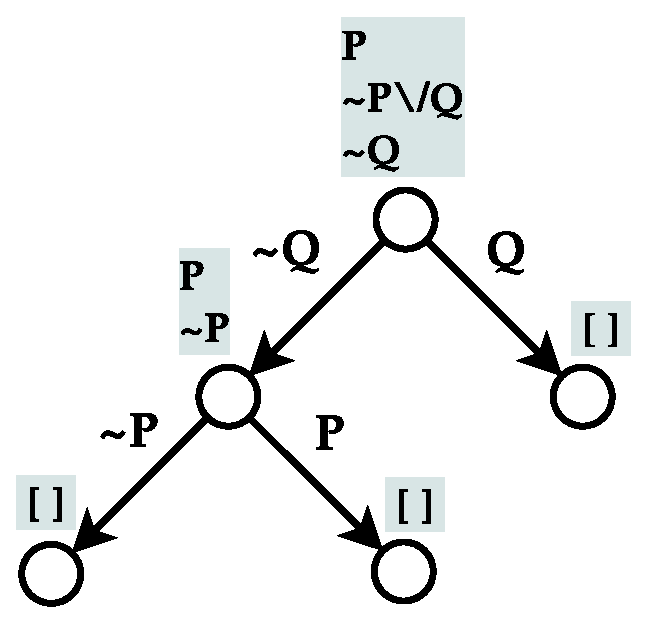
\includegraphics[width=0.35\textwidth]{sat.eps}
  \caption{DPLL算法的的搜索树}
  \label{sat:dpll}
\end{figure}

算法首先尝试$Q$的赋值。当$Q$赋值为真,则与范式中的$\lnot Q$矛盾,因此不可行,回溯;当$Q$赋值为假时,原式变为$P \land (\lnot P \lor \mathrm{false}) \land \mathrm{true}$,即$P \land \lnot P$,然后对$P$做相同的尝试,直到找到一个赋值使得命题成真。

本例经过尝试,发现没有成真的赋值,返回不可满足。

DPLL算法还有不少优化:
\begin{enumerate}
  \item 变量删减:将式子中仅出现正文字或仅出现反文字的变量删除
  \item 变量排序:按照一定的次序搜索,加快剪枝
  \item 约束传播:尽早由部分赋值发现矛盾
  \item 常数时间回溯等
\end{enumerate}
在这些优化下,DPLL算法能够求解变量数上千的SAT问题。

\subsection{证明项的构造}
DPLL算法的证明项构造一般基于归结(resolution)规则构造:
$$\vdash (P \lor Q) \land (\lnot P \lor R) \impl Q \lor R$$
其中$P$、$Q$、$R$都是一阶公式。

当使用归结规则构造DPLL算法的证明项时,需要先对搜索树做若干分析,才能生成证明项,不是很直接。本文提出一个直接生成证明项的方法。

简单地说,这个方法基于如下定理:
$$\alpha' \land E \vdash (P \impl \mathrm{false}) \impl (\lnot P \impl \mathrm{false}) \impl \mathrm{false} $$
其中$\alpha'$是合取范式,$E$是部分赋值的命题编码,$P$是范式中的某一文字。

其意义为:在部分赋值$E$下,若文字$P$赋值为真,最终得到矛盾,且文字$P$赋值为假,最终也得到矛盾,则$\alpha'$不可满足。

应用时,只需要在DPLL搜索树的每个节点按照后序遍历使用即可生成证明。以图\ref{sat:dpll}为例,其生成的证明序列是:
\begin{align*}
  P \land (\lnot P \lor Q) \land \lnot Q \land Q \land P & \vdash \mathrm{false} & (1) & \quad P \land (\lnot P \lor Q) \land \lnot Q \\
  P \land (\lnot P \lor Q) \land \lnot Q \land Q \land \lnot P & \vdash \mathrm{false} & (2) & \quad P \land \lnot P \\
  P \land (\lnot P \lor Q) \land Q \land Q  & \vdash \mathrm{false} & (3) & \quad \text{由定理及(1) (2)}\\
  P \land (\lnot P \lor Q) \land Q \land \lnot Q & \vdash \mathrm{false} & (4) & \quad Q \land \lnot Q \\
  P \land (\lnot P \lor Q) \land Q & \vdash \mathrm{false} & (5) & \quad \text{由定理及(3) (4)}
\end{align*}

\section{命题的规范化}
命题规范化要做的事是将任意的命题化成SAT求解器能够求解的合取范式的形式。

化简过程分为两步:先将命题化简为否定范式(NNF),再将否定范式化为合取范式。

\subsection{规范到否定范式}
规范到否定范式一共要做两件事:消除蕴含词$\impl$;将否定词$\lnot$深入到文字上,并且保证文字前最多只有一个否定词。

从语法结构的观点看,本步骤实际上是由一棵语法树变换到另一棵语法树。由于语法树是由图\ref{sat:stru}构造地定义的,因此只需要考察每一个局部结构的变化情况,再逐级递归即可。

\subsubsection{变换分类}
变换一共分两种情形:A型、B型。图中虚线代表递归时应该看作整体。
\begin{figure}[!h]
\centering
\subfigure[and]{
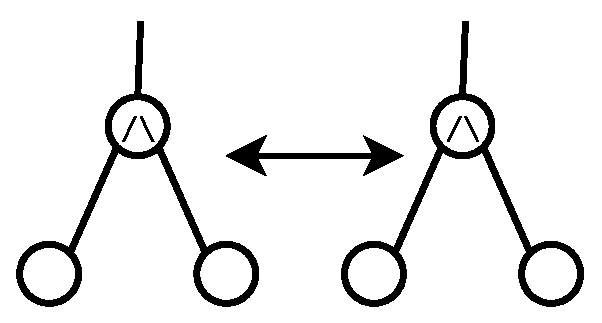
\includegraphics[width=0.27\textwidth]{nnf-and.eps}}
\subfigure[or]{
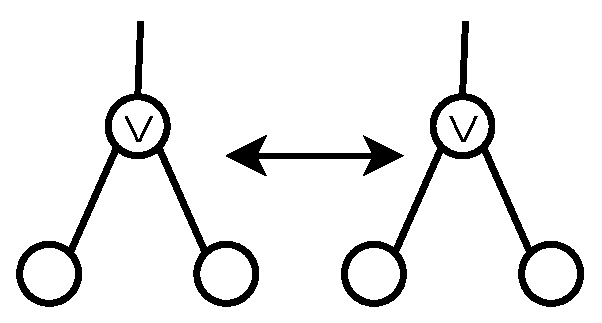
\includegraphics[width=0.27\textwidth]{nnf-or.eps}}
\subfigure[not Y]{
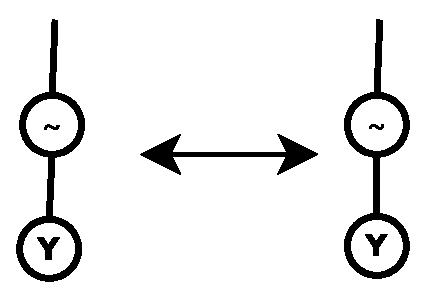
\includegraphics[width=0.19\textwidth]{nnf-np.eps}}
\subfigure[Y]{
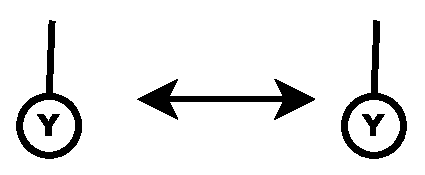
\includegraphics[width=0.19\textwidth]{nnf-p.eps}}
\caption{A型:结构不变}
\end{figure}

\begin{figure}[!h]
\centering
\subfigure[not and]{
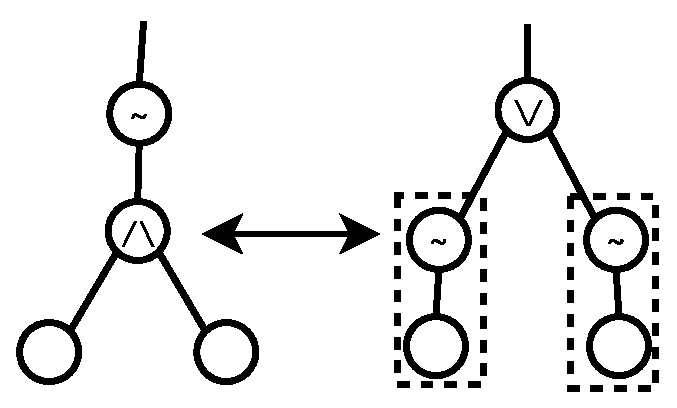
\includegraphics[width=0.32\textwidth]{nnf-nand.eps}}
\subfigure[not or]{
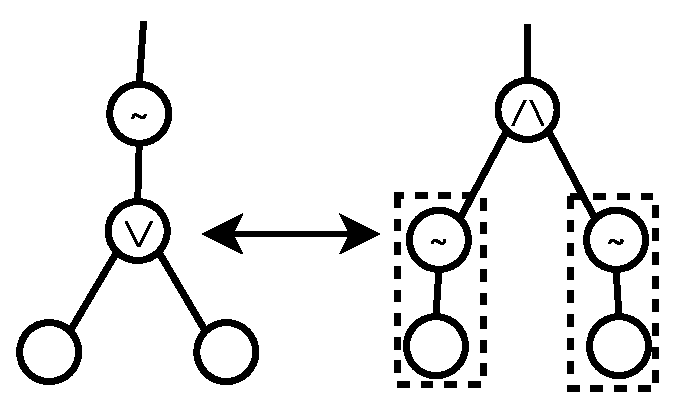
\includegraphics[width=0.32\textwidth]{nnf-nor.eps}}
\subfigure[not not Y]{
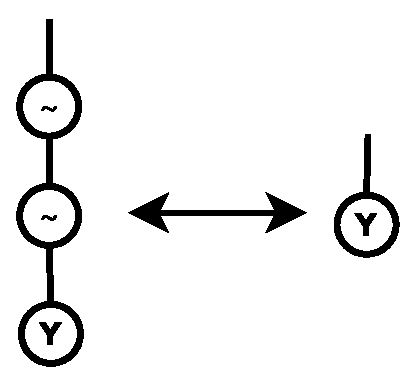
\includegraphics[width=0.19\textwidth]{nnf-nnp.eps}}
\subfigure[imply]{
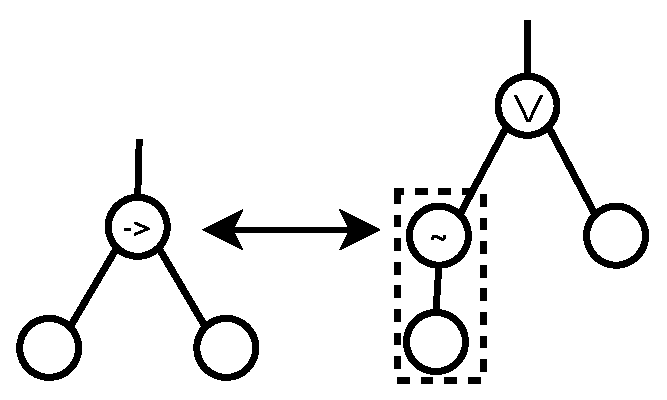
\includegraphics[width=0.32\textwidth]{nnf-imp.eps}}
\subfigure[not imply]{
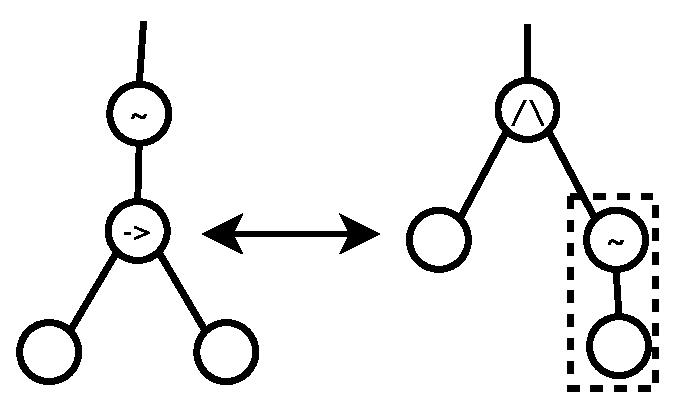
\includegraphics[width=0.32\textwidth]{nnf-nimp.eps}}
\caption{B型:结构改变}
\end{figure}

\subsubsection{证明项构造}
证明项的构造是直接的,只需在递归时引用Coq中预定义的引理即可。

每一种情况对应一个引理,罗列如下。

\paragraph{A型引理}
\begin{verbatim}
Lemma L_and: forall A B C D:Prop, (A<->B)->(C<->D)->((A/\C)<->(B/\D)).
Lemma L_or: forall A B C D:Prop, (A<->B)->(C<->D)->((A\/C)<->(B\/D)).
Lemma L_not: forall A B:Prop, (A<->B)->((~A)<->(~B)).
Lemma iff_p: forall P:Prop, P<->P.
\end{verbatim}

\paragraph{B型引理}
\begin{verbatim}
Lemma iff_nand: forall P Q:Prop, ~(P/\Q) <-> (~P\/~Q).
Lemma iff_nor: forall P Q:Prop, ~(P\/Q) <-> (~P/\~Q).
Lemma iff_nnp: forall P:Prop, ~~P<->P.
Lemma iff_imp: forall P Q:Prop, (P->Q)<->(~P\/Q).
Lemma iff_nimp: forall P Q:Prop, ~(P->Q)<->(P/\~Q).
\end{verbatim}

\subsection{规范到合取范式}
\subsubsection{变换}
从否定范式规范到合取范式是简单的,只需要递归地对公式中的$\lor$做对$\land$的分配律即可。

\subsubsection{证明项构造}
理论上,只要在变换时引用$\lor$对$\land$的分配引理,即可得到合取范式的证明项。但是实践上这样会存在$\land$和$\lor$上交换律和结合律的问题。

例如,$P \lor (Q \lor R)$和$(P \lor Q) \lor R$在日常的非严格的推理中,是看作相同的。但是在Coq系统中却是两个完全不同的类型。若要是类型相等,必须引用结合律。

因此,直接采用分配律后构造证明项后,结果的语法树几乎一定会出现很多“枝杈”,而非规范的右结合树。不是规范形式将会给SAT求解器的证明项构造带来很大负担。

本文提出一个直接由否定范式树生成合取范式每一个的合取支规范形式的方法。

下面以$P \lor (Q \land R)$为例,说明其基本步骤。

\paragraph{从合取范式树抽取合取支}
上式的合取范式为$(P \lor Q) \land (P \lor R)$。容易编写一个递归的过程,抽取出合取支$(P \lor Q)$和$(P \lor R)$并暂存。

\paragraph{决定规范形式}
这里可以根据需要(如根据SAT求解器的内部表示)决定每一个合取支的规范形式,如取为$P \lor Q$和$R \lor P$。

\paragraph{生成合取支的一个析取成分的证明项}
选择$P \lor Q$和$R \lor P$里面一个较好证明的析取支,这里都选择$P$。
即证明:
$$ \vdash P \lor (Q \land R) \impl P $$

由于前件是否定范式,很容易根据$\land$和$\lor$的结构,写一个递归过程,引用Coq如下定理得到证明:
\begin{verbatim}
Lemma and_ind : forall A B P : Prop, (A -> B -> P) -> A /\ B -> P.
Lemma or_ind : forall A B P : Prop, (A -> P) -> (B -> P) -> A \/ B -> P.
\end{verbatim}

\paragraph{补齐其余部分}
写一个递归过程,引用下列Coq定理,补齐合取支的其他部分。
\begin{verbatim}
Lemma or_introl : forall A B : Prop, A -> A \/ B.
Lemma or_intror : forall A B : Prop, B -> A \/ B.
\end{verbatim}
本例中,可用\texttt{or\_introl}由$P$得到$P \lor Q$;用\texttt{or\_intror}由$P$得到$R \lor P$。

至此,我们得到了否定范式到合取范式每一个合取支的规范形式的证明项。并且,由于SAT求解器实际实现时接收的就是合取范式合取支。因此,不必再用\texttt{conj}引理得到合取范式的证明项。

本文提出的这种方法,相当于把公式的化简、规范化、拆项三步放到了一步之中,减少了证明项的大小。
